% fig01_geqoe_state_vector.tex
% Standalone TikZ: GEqOE state vector elements on the physical orbit
\documentclass[tikz,border=5pt]{standalone}
\usepackage{amsmath,amssymb}
\usetikzlibrary{arrows.meta,calc,decorations.pathreplacing,decorations.markings,
                positioning,3d}

\definecolor{accent}{RGB}{0, 100, 170}
\definecolor{highlight}{RGB}{200, 60, 30}
\definecolor{darkgreen}{RGB}{0, 120, 60}
\definecolor{earthblue}{RGB}{40,80,150}
\definecolor{orbitgray}{RGB}{100,100,100}

\begin{document}
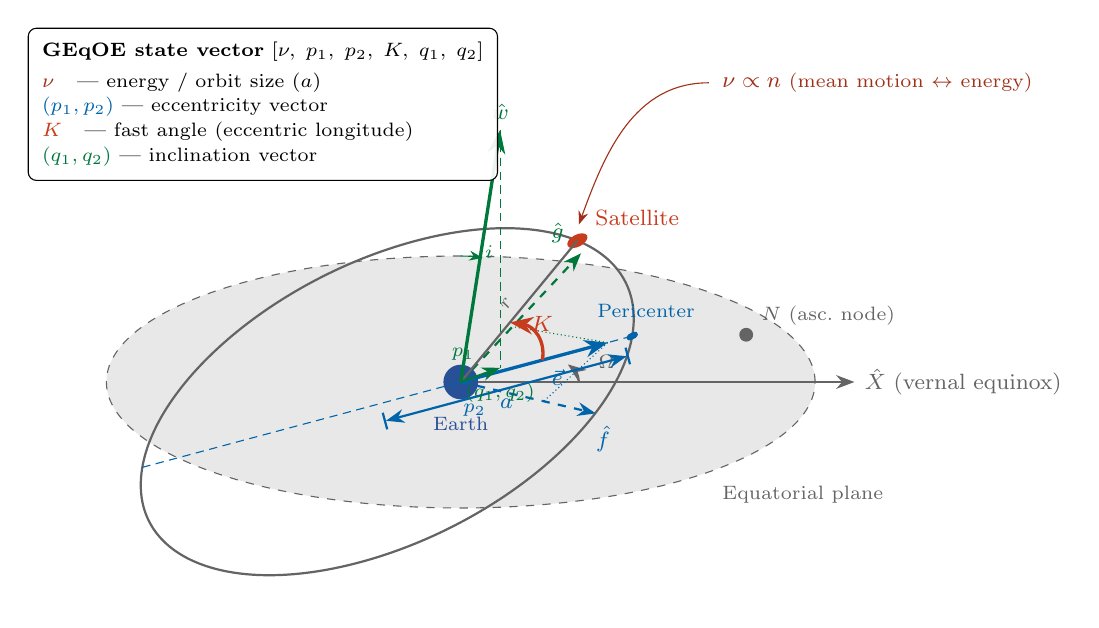
\begin{tikzpicture}[
    >=Stealth,
    font=\footnotesize,
    scale=1.0,
  ]

  %% ── Projection parameters ──
  % We simulate a 3D perspective by skewing
  % Equatorial plane basis vectors (projected)
  \pgfmathsetmacro{\eqXx}{1.0}   \pgfmathsetmacro{\eqXy}{0.0}
  \pgfmathsetmacro{\eqYx}{0.45}  \pgfmathsetmacro{\eqYy}{0.35}
  % Orbital plane basis vectors (tilted ~35 deg from equatorial)
  \pgfmathsetmacro{\opXx}{1.0}   \pgfmathsetmacro{\opXy}{0.15}
  \pgfmathsetmacro{\opYx}{0.3}   \pgfmathsetmacro{\opYy}{0.75}

  %% ── Equatorial plane (gray ellipse) ──
  \begin{scope}[opacity=0.15]
    \fill[orbitgray] (0,0) ellipse (4.5cm and 1.6cm);
  \end{scope}
  \draw[orbitgray, thin, dashed] (0,0) ellipse (4.5cm and 1.6cm);
  \node[orbitgray, anchor=north west] at (3.2, -1.2) {\scriptsize Equatorial plane};

  %% ── Reference direction (vernal equinox) ──
  \draw[->, thick, orbitgray] (0,0) -- (5.0, 0)
    node[right] {$\hat{X}$ (vernal equinox)};

  %% ── Earth at center ──
  \fill[earthblue] (0,0) circle (0.22);
  \node[earthblue, anchor=north, yshift=-3pt] at (0, -0.22) {\scriptsize Earth};

  %% ── Ascending node ──
  \pgfmathsetmacro{\nodeAngle}{25}
  \pgfmathsetmacro{\nodeR}{4.0}
  \coordinate (Node) at ({\nodeR*cos(\nodeAngle)}, {\nodeR*sin(\nodeAngle)*0.355});
  % Direction in equatorial plane at angle Omega
  \coordinate (NodeDir) at ({cos(\nodeAngle)}, {sin(\nodeAngle)*0.355});
  \fill[orbitgray] (Node) circle (2.5pt);
  \node[orbitgray, anchor=south west, xshift=2pt] at (Node) {\scriptsize $N$ (asc.\ node)};
  % Omega arc
  \draw[orbitgray, thick, ->] (1.5, 0) arc[start angle=0, end angle=\nodeAngle,
    x radius=1.5cm, y radius=0.53cm];
  \node[orbitgray] at (1.85, 0.25) {\scriptsize $\Omega$};

  %% ── Orbital ellipse ──
  % Orbit: e ~ 0.3, semi-major a = 3.0 cm, tilted
  % We draw the orbit in a rotated/tilted frame
  \pgfmathsetmacro{\sma}{3.0}     % semi-major axis in cm
  \pgfmathsetmacro{\ecc}{0.30}    % eccentricity
  \pgfmathsetmacro{\smb}{\sma*sqrt(1-\ecc*\ecc)} % semi-minor axis
  \pgfmathsetmacro{\focalShift}{\sma*\ecc}        % focus offset

  % The orbit plane is tilted: we draw in a scope with appropriate transform
  % Orbit is rotated by argument of ascending node + inclination tilt
  \begin{scope}[
    cm={\opXx,\opXy,\opYx,\opYy,(0,0)},  % tilted orbital plane
    rotate=10,  % argument of node rotation in orbital plane
  ]
    % Draw the orbit ellipse (center at (-focalShift, 0) so focus is at origin)
    \draw[orbitgray, thick] (-\focalShift, 0) ellipse ({\sma} and {\smb});

    %% ── Semi-major axis line ──
    \draw[accent, thin, densely dashed]
      ({-\focalShift - \sma}, 0) -- ({-\focalShift + \sma}, 0);
    % Dimensioned line for 'a'
    \draw[accent, thick, |<->|] (-\focalShift, -0.35) -- ({\sma - \focalShift}, -0.35)
      node[midway, below, accent] {$a$};

    %% ── Pericenter mark ──
    \coordinate (Peri) at ({-\focalShift + \sma}, 0);
    \fill[accent] (Peri) circle (2pt);
    \node[accent, anchor=south, yshift=3pt, xshift=5pt] at (Peri)
      {\scriptsize Pericenter};

    %% ── Eccentricity vector ──
    % From focus (origin) toward pericenter
    \pgfmathsetmacro{\evecLen}{1.8}
    \draw[->, accent, very thick] (0,0) -- (\evecLen, 0)
      node[pos=0.6, below, xshift=3pt] {$\vec{e}$};

    %% ── Equinoctial axes f-hat and g-hat ──
    % f-hat and g-hat are in the orbital plane, f along reference
    % For illustration, let omega_tilde ~ 35 deg
    \pgfmathsetmacro{\omtilde}{35}
    \pgfmathsetmacro{\fhatLen}{2.2}
    % f-hat direction (in orbital plane, from ascending node direction)
    \draw[->, accent, thick, dashed]
      (0,0) -- ({\fhatLen*cos(-\omtilde)}, {\fhatLen*sin(-\omtilde)});
    \node[accent, anchor=north] at ({\fhatLen*cos(-\omtilde)+0.1},
      {\fhatLen*sin(-\omtilde)-0.1}) {$\hat{f}$};
    % g-hat perpendicular to f-hat
    \draw[->, darkgreen, thick, dashed]
      (0,0) -- ({\fhatLen*cos(90-\omtilde)}, {\fhatLen*sin(90-\omtilde)});
    \node[darkgreen, anchor=south east] at ({\fhatLen*cos(90-\omtilde)-0.1},
      {\fhatLen*sin(90-\omtilde)+0.05}) {$\hat{g}$};

    %% ── p1, p2 decomposition ──
    % p2 = e cos(omega_tilde) along f-hat
    \pgfmathsetmacro{\ptwoval}{\ecc*cos(\omtilde)*5.5}
    \pgfmathsetmacro{\poneval}{\ecc*sin(\omtilde)*5.5}
    % Dashed projection lines
    \draw[accent, thin, densely dotted]
      (\evecLen, 0) -- ({\ptwoval*cos(-\omtilde)}, {\ptwoval*sin(-\omtilde)});
    \draw[darkgreen, thin, densely dotted]
      (\evecLen, 0) -- ({\poneval*cos(90-\omtilde)}, {\poneval*sin(90-\omtilde)});
    % Labels
    \node[accent, anchor=north, yshift=-1pt, xshift=-10pt]
      at ({0.5*\ptwoval*cos(-\omtilde)}, {0.5*\ptwoval*sin(-\omtilde)})
      {\scriptsize $p_2$};
    \node[darkgreen, anchor=east, xshift=-1pt]
      at ({0.5*\poneval*cos(90-\omtilde)}, {0.5*\poneval*sin(90-\omtilde)})
      {\scriptsize $p_1$};

    %% ── Satellite position ──
    % True anomaly f ~ 60 deg from pericenter
    \pgfmathsetmacro{\trueAnom}{60}
    \pgfmathsetmacro{\rsat}{\sma*(1-\ecc*\ecc)/(1+\ecc*cos(\trueAnom))}
    \coordinate (Sat) at ({\rsat*cos(\trueAnom)}, {\rsat*sin(\trueAnom)});
    \fill[highlight] (Sat) circle (3.5pt);
    \node[highlight, anchor=south west, xshift=3pt, yshift=2pt] at (Sat)
      {\footnotesize Satellite};

    %% ── K angle (eccentric longitude) ──
    % Arc from reference direction (f-hat direction in the orbital plane)
    % to the satellite, measured from vernal equinox projection
    % For visual clarity, show arc from x-axis to satellite
    \pgfmathsetmacro{\Kangle}{\trueAnom}
    \draw[highlight, very thick, ->]
      (1.0, 0) arc[start angle=0, end angle=\Kangle,
      x radius=1.0cm, y radius=1.0cm];
    \node[highlight, anchor=south west] at ({0.8*cos(\Kangle/2)},
      {0.9*sin(\Kangle/2)}) {$K$};

    %% ── r line ──
    \draw[orbitgray, thick] (0,0) -- (Sat)
      node[midway, above, sloped, orbitgray] {\scriptsize $r$};
  \end{scope}

  %% ── nu annotation ──
  \node[highlight!80!black, anchor=west] at (3.2, 3.8)
    {$\nu \propto n$ \scriptsize (mean motion $\leftrightarrow$ energy)};
  \draw[->, highlight!80!black, thin] (3.15, 3.8) to[out=180, in=70] (1.5, 2.0);

  %% ── Orbit normal / q1,q2 ──
  % Orbit normal vector
  \draw[->, darkgreen, very thick] (0,0) -- (0.5, 3.2)
    node[anchor=south] {\footnotesize $\hat{w}$};
  % Show q1, q2 as projection onto equatorial plane
  \draw[darkgreen, densely dashed, thin] (0.5, 3.2) -- (0.5, 0.18);
  \draw[->, darkgreen, thick] (0,0) -- (0.5, 0.18);
  \node[darkgreen, anchor=north, yshift=-2pt] at (0.5, 0.18)
    {\scriptsize $(q_1, q_2)$};
  % Inclination angle
  \draw[darkgreen, thin, ->] (0, 1.6) arc[start angle=90, end angle=80,
    radius=1.6cm];
  \node[darkgreen, anchor=west, xshift=1pt] at (0.15, 1.65) {\scriptsize $i$};

  %% ── Legend box ──
  \node[draw, rounded corners=3pt, fill=white, fill opacity=0.92, text opacity=1,
        inner sep=5pt, anchor=north west, font=\scriptsize,
        align=left] at (-5.5, 4.5) {%
    \textbf{GEqOE state vector} $[\nu,\; p_1,\; p_2,\; K,\; q_1,\; q_2]$\\[3pt]
    \textcolor{highlight!80!black}{$\nu$} ~~--- energy / orbit size ($a$)\\[1pt]
    \textcolor{accent}{$(p_1, p_2)$} --- eccentricity vector\\[1pt]
    \textcolor{highlight}{$K$} ~~--- fast angle (eccentric longitude)\\[1pt]
    \textcolor{darkgreen}{$(q_1, q_2)$} --- inclination vector
  };

\end{tikzpicture}
\end{document}
